\documentclass[preprint,authoryear,5p]{elsarticle} 
\usepackage{amssymb, amsmath, amsthm, microtype, booktabs, dcolumn} 
\usepackage{pgfplots} 
\usepackage{pgfplotstable} 
\usepgfplotslibrary{dateplot} 
\usetikzlibrary{plotmarks} 
\usepackage[pdftex,colorlinks=true,citecolor=magenta,urlcolor=magenta,pdfstartview=FitH]{hyperref} \pdfcompresslevel=9 \hypersetup{pdftitle={How to Write a Shiny Paper}, pdfauthor={Anonymous}} 
\def\bibsection{
\section*{References}}

%\journal{}
\begin{document}
\begin{frontmatter}
	
	\title{How to Write a Shiny Paper\tnoteref{titlelable}} \tnotetext[titlelable]{This paper is written for those STREEM or TSCM master-students who want to write a master thesis in the form of an article and who like to use more sophisticated tools to do so. Note that I do not aim to discuss writing skills, but instead aim to discuss tools for better presentation of research results. Why by the way an Elsevier type of article? Well, it doesn't matter that much, but I for myself appreciate the format. And it is created by people who actually understand typesetting. So, for the moment we do not want to reinvent the wheel and knick Elsevier's style file. Welcome to the realm of open source!} 
	\author{Thomas de Graaff} \ead{t.de.graaff@vu.nl} \ead[url]{www.thomasdegraaff.net} \address{Department of Spatial Economics, Vrije Universiteit}
	\begin{abstract}
		This papers explains what tools you need to write a paper that (in this case) looks like an Elsevier article. The underlying theory, however, of why certain tools are better than others is applicable to almost all types of output (e.g., theses, papers, presentations, posters, and articles in any other format). With this paper I hope that (advanced) students are willing to give the tools discussed a try---even if the learning curve in the beginning might be quite steep. 
	\end{abstract}
	\begin{keyword}
		Automation, workflow, text files, \LaTeX \sep citation manager 
	\end{keyword}
\end{frontmatter}

\section{Why bother?} Well, first of all, you obviously want to write a shiny paper; a paper that looks really nice, is easy to read, and where each of the elements---including references, mathematics, tables and figures---have a consistent look. And the point is: this is far more difficult (though possible) with conventional---read Word---tools. Secondly, and more persuasive perhaps, conventional proprietary tools do not lend themselves easily to customisation and automisation. For instance, it is rather difficult to directly import Stata output in tables in Word; it always has to go indirectly, or using Excel or using Rich Text Format (rtf). 

Although this tutorial advocates the use of some particular tools, it actually does not matter that much as long as they are able to use plain text files. Plain text files namely have a number of advantages over other type of files; they are transparent (you can always read and edit them), portable (they are the same on each system) and they are not likely to become obsolete in the coming decades. And a lot of files or even tools just consists of plain text files, such as HTML code, most open source tools and Stata `do' files. Most proprietary tools have formats that are not made of plain text, such as Word, Excel, or powerpoint (as well as the Stata data format by the way). This makes them not only less flexible but the risk of getting stuck in an obsolete data format\footnote{The case of the late but much beloved wordprocessor `Word Perfect' comes to mind.} is nontrivial, while output is not similar on each operation system or even across versions. 

\section{Managing workflow} It is difficult to define what `good workflow' is, but it certainly has to satisfy each of the following elements to some degree:\footnote{Almost directly taken from this \href{http://blog.revolutionanalytics.com/2010/10/a-workflow-for-r.html}{blog}; another wonderful source is \citet{Healy2013}.} 
\begin{enumerate}
	\item Transparency: A good workflow organizes the elements of the project logically and clearly, to make it easy for an observer (including yourself) to understand how the pieces come together. 
	\item Maintainability: A good workflow makes it easy to modify and adapt the project. Standardized script names and good commenting practices are key here. 
	\item Modularity: A good workflow encapsulates discrete tasks into separate components (e.g. scripts), so that it's always clear where modifications need to be made (and only made in one place), and components are re-usable for other projects. 
	\item Portability: A good workflow makes it easy to move the project to another system, or hand it over to another person to work on, in such a way that it can still easily be run elsewhere. (By using relative (not absolute) pathnames is one example.) 
	\item Reproducibility: A good workflow makes it easy for you, or others, to reproduce your results. 
	\item Efficiency: A good workflow saves you time, by making it easier to work on the project, and by automating as much of the process as possible. 
\end{enumerate}

\section{\LaTeX \: instead of `What You See Is What You Get' tools} Word and Powerpoint are usually described as `What You See Is What You Get' (WYSIWYG) tools. But what you get is sometimes below par. That's why some advocate the use of `What You Mean Is What You Get' (WYMIWYG) tools. And these tools usually apply to markup languages. The most famous of these languages is HTML, which is just a bunch of code describing how text \emph{should} look like on screen. 

\LaTeX \ is a markup language as well, that just consists of code describing how a text should look like (on paper, screen or beamer). Instead of a word processing program, \LaTeX \ is a typesetting program that determines for itself how words, sentences, paragraphs, etcetera, are placed on paper, slide or pdf file. Actually, \LaTeX{} is a program (or compiler) that is fed by an input text file. Novice users find this most difficult; everything should be more or less coded. However, this allows for great flexibility, transparency, portability, and even efficiency. The same code can namely be used for papers, presentations and posters alike.

Where \LaTeX \ truly shines is in the scientific domain.\footnote{But not only given the nice examples on this \href{http://www.tug.org/texshowcase/}{website}.} If one wants to consistently typeset text, figures, tables, references and especially equations, nothing outperforms {\LaTeX}.\footnote{\LaTeX \ itself is just a bunch of macros around \TeX, a typesetting program devised by the notorious computer scientist Donald Knuth. \LaTeX\ was created by Leslie Lamport in 1984 and \TeX was created in 1978. Yes, it is that old.} And in the end, that is what you want to do: write a nice shiny paper. 

\subsection{Where to get it?}

One of the nice things about {\LaTeX} is that it works on (almost) all operating systems. To get it to work you need two things: the program itself and an editor. For windows this usually means downloading \href{http://miktex.org/}{MikTeX} and \href{http://www.texniccenter.org/}{TeXNicCenter} or \href{http://www.tug.org/texworks//}{TeXworks}. On a mac, both program and editor (and lots more) can be downloaded from the \href{http://tug.org/mactex/}{MacTex} site with its celebrated TexShop editor. 

\subsection{I got it, and now what?}

There are numerous tutorials on the web, but I recommend to first take a look at the \href{http://latex-project.org/}{latex project} website, which comes with a whole bunch of tutorials (and yes, they are all free). 

Without really going into the nitty gritty of this language, let's write our quintessential 'hello world' program. 
\begin{verbatim}
	% hello.tex - A very simple LaTeX example!
	\documentclass{article} 
		\begin{document} 
				Hello World! 
		\end{document} 
\end{verbatim}
with the following output (but then as a separate document):
\newline
\newline
Hello World!
\newline
\newline
Okay, this perhaps doesn't look like much, but it actually contains quite some interesting elements. First, lines starting with a \% sign are used as comments. Second, you first have to specify what kind of text you are typesetting (in this case an article). And finally, every element needs a `begin' and an `end' (just as we all do). In this case, the whole document needs to be specified. Things start to heat up a bit, when you add formulas such as when we add the following lines to our simple example 
\begin{verbatim}
	You know, I just discovered that: 
	\begin{equation}
		E = mc^2 
	\end{equation}
\end{verbatim}
with the following output: 
\newline 
\newline You know, I just discovered that: 
\begin{equation}
	E = mc^2 
\end{equation}

Where again, we need to put something between a `begin' and an `end' statement, in this case the equation. The code for equations (or math mode) is remarkably similar to that of Excel and does not take long to get used to. If one wants to have mathematics displayed inline it usually is best to use dollar signs such as:\footnote{It takes some time to get used to all the mathematics commands. Luckily, the internet is full of cheatsheets, wikis and manuals about this, such as \href{http://en.wikibooks.org/wiki/LaTeX/Mathematics}{this}.} 
\begin{verbatim}
	$\frac{d x}{d y} = -\frac{
	\partial u(x,y)/
	\partial y} {
	\partial u(x,y)/
	\partial y}$ 
\end{verbatim}
which displays as: $\frac{d x}{d y} = -\frac{
\partial u(x,y)/
\partial y} {
\partial u(x,y)/
\partial x}$. Before we now set off, there is one thing you need to know, and that is the use of packages and classes. Because {\LaTeX} consists of macros it is completely adjustable and that is exactly what people have done and where the strength of the application can be found; in user-written packages and classes. For example, when you want your paper to look like an Elsevier article (and in this case you do), then use the \emph{elsarticle} class instead of the \emph{article} class.\footnote{This class usually is already installed or can be found on Elsevier's website or on the repository of {\LaTeX} packages---\href{www.ctan.org}{www.ctan.org}. On \href{http://www.elsevier.com/author-schemas/latex-instructions}{Elsevier's} website you can download as well a template, which comes in handy when starting a paper.} 

Usually, the best way of learning this is by looking at examples of others. Take a look, e.g., at the source code for this pdf file. At the top it says use the \emph{elsarticle} with some options (e.g., the \emph{5p} option states that the text should be typesetted in two-columns---\emph{3p} would indicate one column). Below that I load a bunch of packages which usually have something to do with how to display tables, mathematics, links and references. Then there is some front matter stuff, such as authors, title, addresses and an abstract, after which the main text follows, nicely divided in sections and subsections. The only further thing handy to know in this stage is that an open line indicates a new paragraph. 

\subsection{Ok, but how about Tables?}

One of the more painful things to do in \LaTeX{} is composing tables. That's why you should never do so. Instead, you should let other applications do the trick for you. For instance, R and Stata can easily transform regression output to a \LaTeX{} format which can be directly inserted in your \LaTeX{} file---remember, every element here is a text file.\footnote{Typical packages for Stata are outtex and outreg2 and for R xtable and stargazer.} The following table gives an example and displays the output of a regression model of car characteristics on car mileage with two specifications. 

\input{results.tex}

This table is created with only four commands, two to do the regressions in Stata, one to write the output in two columns to a file in \LaTeX \ format, and the last to import the table in this text file. This approach has numerous advantages, namely: it is very efficient, it is not error prone\footnote{Most mistakes in scientific research are made in pre- or post analysis operations; a.k.a. fumbling a bit with Excel and typing over your results.} and you can very easily change the results for different samples, specifications or functional forms.

\subsection{And what about figures, diagrams and graphs?}

Fortunately, figures, diagrams and graphs are much easier to handle in {\LaTeX} than tables. And, as long as you want to draw something in a schematic way, you can even make your own diagrams and graphs using a couple of additional packages!

\subsubsection{Figures}

Because the output of {\LaTeX} is already in pdf format it can easily incorporate figures from many format, such as the printer languages .pdf and .ps, but as well .jpeg and others. For example, this command: 
\begin{verbatim}
	\begin{figure}[h!]
		\center 
		
\includegraphics[width=0.3\textwidth] 
		{ligatures_latex} \caption{Correct 
		use of ligatures in \LaTeX (Source: 
		\href{http://nitens.org/ taraborelli/latex}
		{Taborelli})} 
	\end{figure}
\end{verbatim}
produces Figure (\ref{ligatures}):
\begin{figure}[h!] 
	\center 
	
\includegraphics[width=0.3
	\textwidth]{ligatures_latex} \caption{Correct use of ligatures in {\LaTeX} (Source: \href{http://nitens.org/taraborelli/latex}{Taborelli})} 
	\label{ligatures}
\end{figure}

\noindent The command \verb+h!+ states that the figure should very explicitly (the \verb+!+ command) be placed about here (the \verb+h+ command).

When captions are incuded they are correctly numbered and size and position of the figure (even across columns) can easily be adjusted. 

\subsubsection{Graphs \& plots}

Creating structured graphs and plots based on data is rather straightforward with the use of appropriate packages. In this case the packages \emph{tikz} and \emph{pgfplots} come in very handy (they also come with very extended manuals full of examples). Suppose that we are interested in depicting the outcomes of a meta-analysis concerning the relation between the elasticity of between migration and imports on the one hand and the elasticiy between the migration and exports on the other hand. Moreover, the original results have been written to a simple text file.\footnote{The text file is named `migrationFDI.txt' and is generously provided by Masood Gheasi. The original research is documented in \citet{Ghen2012}.} Then with a couple of commands (I refer to the source of this file to avoid too much clutter) one gets Figure (2). 

\begin{figure}[h!]
	 \center 
	\begin{tikzpicture}
		\begin{axis}
			[xlabel={Migration elasticity of imports}, ylabel={Migration elasticity of exports}, xmax = 3.5,ymax=3.5, x = 1cm, y=1cm, xmin = -2, ymin=-2, legend pos= south east] \addplot[x=import, y = export,scatter, only marks] table {migrationFDI.txt}; \addlegendentry{Estimate} \addplot[blue, mark=none, thick] table[ x=import,y={create col/linear regression={y=export}}]{migrationFDI.txt}; \addlegendentry{slope $\pgfmathprintnumber{\pgfplotstableregressiona}$} 
		\end{axis}
	\end{tikzpicture}
	\caption{A meta-analysis on the elasticity between migration and trade} 
\end{figure}

One of the main advantages in doing it as such, is that typesetting remains consistent. This also applies to symbols and equations in the title(s), legends, tick-marks or even as labels within the graph. Another large advantage is that the slope estimate is automatically generated. Thus, if additional observations (research outcomes) are added to the meta-analysis, then Figure (2) will be automatically updated. 

\subsubsection{Diagrams} 

The \emph{tikz} package  can as well be used for drawing diagrams of your own.\footnote{There are other ways of creating structured diagrams, both within the and outside the {\LaTeX} environment. An exampple of the latter is the metapost language.} This requires a bit more code and thought but is able to deliver very sharp structured diagrams with consistent typesetting. And, if you have done it once, you can always reuse the code (e.g., for presentation, handouts or class-slides). Very good sources on the internet are \href{http://www.texample.net/tikz/examples/}{Tikz examples} and the blog of Kevin Goulding \href{http://thetarzan.wordpress.com/2011/06/19/tikz-for-economists-a-how-to-guide-with-examples/}{Tikz for economist}. Once more, the \href{http://paws.wcu.edu/tsfoguel/tikzpgfmanual.pdf}{manual} of Tikz is as well quite good and rather elaborate. 

One of my own examples is a diagram of an Edgeworth-Box, which is---as you might know---rather painfull to do in Excel. Figure \ref{Ebox} has been coded to be used in the second year's course Regional Economics. And the particular advantage of doing it like such is that the parameters (in this case, the endowments of both capital and labour and the parameters of the prodution function of both countries $A$ and $B$) are fully adjustable, which might be particular useful for variations in examinations and assignments. 
\begin{figure}[h!] 
	\center 
	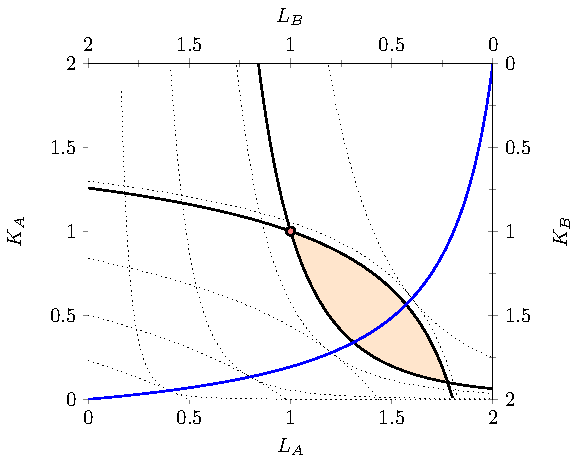
\includegraphics[width=0.45
	\textwidth]{EdgeworthBox} \caption{Tikz Diagram of an Edgeworth Box (Source: own code)}
	\label{Ebox}
\end{figure}

\section{Always use a citation manager}

The first thing I do recommend to all students (and researchers) is to use a citation manager. Even when using applications such as Microsoft Word (the horror\ldots). This is one tool that immediately delivers in terms of efficiency. Even if initially setting up a database with references might be time-consuming it still pays off in later stages. The point is that you only once have to type in a reference within a database. Later on you can always use this reference within the text and the reference or bibliography list should be automatically generated. And there are even reference managers that can import folders with articles in pdf format and automatically generate a reference database. 

Within the {\LaTeX} environment, the application BibTeX is usually used. There are separate editors for this system, but the easiest way is using a more generic reference manager (the free Mendeley application comes to mind) that can write files to .bib files (the BibTeX format) or incorporate references directly within Microsoft Word. In this way, your remain as flexible as possible. 

\section{From here \ldots into the abyss}

Right. so we know now how to write a shiny paper with tables, references and perhaps even customated diagrams. Would that be it? No, it is just the start of a completely automated, customated, transparent and (hopefully) more efficient workflow. For that you need a set of tools that are complementary to each other. And fortunately, most of them are. However, choose your tools carefully. All of them are costly in terms of learning curves and there is only so much time available to you. Having said that, there are a couple of choices you might want to make eventually, of which the following three are probably most important. 

First of all, the choice of editor. Of course, TexShop or TeXNicCenter are nice editors, but are mostly suited for {\LaTeX}. In the end, you might want to use a more versatile editor. One editor capable of editing R scripts, stata do files, html code, etcetera. All with proper highlighting and a consistent set of shortcuts. I am not saying which editor you should use. Too many have found their demise at the \href{http://en.wikipedia.org/wiki/Editor_war}{editor war}. There are many good (and free) ones out there. And even the ones you have to pay for are well worth the money. Pick up and stick to it for some time. For OsX there is now a free version of Textmate, which is quite good. And cross platforms, sublime is another editor well worth looking into. If you really want to go nerdy, opt for Emacs of Vi(m). Longstanding, very capable (and fast) editors. However, be aware of a steep learning \href{http://www.terminally-incoherent.com/blog/wp-content/uploads/2006/08/curves.jpg}{curve}. 

Second, as already hinted upon, the combination of {\LaTeX} with statistical programs such as Stata and R is a killer app. If one has to choose, I would advise you to invest in R. Stata is more an econometric package, while R is much more statistical. And the userbase of the latter is much larger than the former, ensuring that with R most problems dealing with statistics (or even GIS) have already been dealt with. Moreover, there is a very nice editor, Rstudio, able to integrate them both. Heck, you can even weave {\LaTeX} and R code together (called Sweave or Knitr) with mindblowing results. This comes rather close to what Donald Knuth coined literate programming: the simultaneous generation of the output of both text as analysis.

Third, and finally, think very carefully about backup programs. You know, you never need it until you really need it. The first advise is to always use an external disk with a backup application (such as Time Machine on OsX). Secondly, having some of your applications (especially your code, and thus text, files) somewhere in the cloud has additional benefits. Apart from a backup advantage, it also facilitates working together on a project. The best known of these applications is Dropbox, although cooperation using this is still a bit cumbersome. Another, more nerdy, example is using Git, which is a full blown distributed revision control and source code management system, created by Linus Torvards (that guy from Linux). It takes some time to get use to, but in the end it grows on you and becomes not only easier to use, but makes you in the end even more efficient. 

As a last example about complementarity, the before mentioned Rstudio application does not only edit {\LaTeX} and R, but is able as well to set up a Git repository system. In the end, it comes all together. 

\section{Some final thoughts}

This might all seem a bit daunting. The best advise for novices would be: start one step at a time (``A journey of a thousand miles begins with a single step'', Lao-tzu). In this case this simply means that you start with a template file (such as that from the Elvesier article class), incorporate or copy in some text, divide it by section and subsection headers and see whether it works. 

Granted, the learning curves of most of these tools are rather steep (except for that of using citation managers---you really should use them). However, it does pay-off in the end. And most of these tools have the fortunate feature to be very \emph{complementary} to each other. A good example is making slides. There is a package out there called beamer, which allows you to create slides from your text. This basically means, that all your codes used for your paper can be used again for your slides (within a {\LaTeX} context, so equations won't fly all over the slide as sometimes happens with more conventionals presentation programs). If you know one application really well, it becomes easier to understand others or even use the same commands. And there are quite a few applications or languages out there that work with text files and are very handy for a researcher---HTML, Markdown, Latex, scripting languages from Stata and R and even languages as Ruby and Python come to mind. The latter, for example, is the native language of ArcGis scripts. 

Obviously, this paper is way too short to do justice to them. However, starting with {\LaTeX} would be a good introduction to a more customated and automated workflow.

\bibliographystyle{elsarticle-harv} 
\bibliography{ref}

\end{document} 
